\chapter{Optimization Problem}

\section{Definition of Optimization Problem}

\begin{definition}[1.1][Optimization Problem]
    In an \textbf{optimization problem}, we minimize or maximize a function value, possibly subject to constraints.

    $$
    \begin{array}{ll}
    \underset{\theta \in \mathbb{R}^{p}}{\operatorname{minimize}} & f(\theta) \\
    \text { subject to } & h_{1}(\theta)=0, & \cdots & , \ h_{m}(\theta)=0, \\
    & g_{1}(\theta) \le 0, & \cdots & , \ g_{n}(\theta) \le 0
    \end{array}
    $$

    \begin{itemize}
        \item Decision variable: $\theta$
        \item Objective function: $f$
        \item Equality constraint: $h_{i}(\theta)=0$ for $i=1, \ldots, m$
        \item Inequality constraint: $g_{j}(\theta) \leq 0$ for $j=1, \ldots, n$
    \end{itemize}
\end{definition}

In machine learning (ML), we often minimize a "loss", but sometimes we maximize the "likelihood".
In any case, minimization and maximization are equivalent since

$$
\text { maximize } f(\theta) \quad \Leftrightarrow \quad \text { minimize }-f(\theta).
$$

\begin{definition}[1.2][Feasible Point and Constraints]
    $\theta \in \mathbb{R}^{p}$ is a \textbf{feasible point} if it satisfies all constraints:

    $$
    \begin{array}{cc}
    h_{1}(\theta)=0 & g_{1}(\theta) \leq 0 \\
    \vdots & \vdots \\
    h_{m}(\theta)=0 & g_{n}(\theta) \leq 0
    \end{array}
    $$

    Optimization problem is \textbf{infeasible} if there is no feasible point.

    An optimization problem with no constraint is called an \textbf{unconstrained optimization problem}. Optimization problems with constraints is called a \textbf{constrained optimization problem}.
\end{definition}

\begin{definition}[1.3][Optimal Value and Solution]
    \textbf{Optimal value} of an optimization problem is

    $$
    p^{\star}=\inf \left\{f(\theta) \mid \theta \in \mathbb{R}^{n}, \theta \text { feasible }\right\}
    $$

    \begin{itemize}
        \item $p^{\star}=\infty$ if problem is infeasible
        \item $p^{\star}=-\infty$ is possible
        \item In ML, it is often a priori clear that $0 \leq p^{\star}<\infty$.
    \end{itemize}

    If $f\left(\theta^{\star}\right)=p^{\star}$, we say $\theta^{\star}$ is a \textbf{solution} or $\theta^{\star}$ is \textbf{optimal}.\\
    A solution may or may not exist, and a solution may or may not be unique.
\end{definition}

\section{Examples of Optimization Problem}

\begin{example}[1.4][Curve Fitting]
    Consider setup with data $X_{1}, \ldots, X_{N}$ and corresponding labels $Y_{1}, \ldots, Y_{N}$ satisfying the relationship

    $$
    Y_{i}=f_{\star}\left(X_{i}\right)+\text { error }
    $$

    for $i=1, \ldots, N$. Hopefully, "error" is small. True function $f_{\star}$ is unknown.

    Goal is to find a function (curve) $f$ such that $f \approx f_{\star}$.
\end{example}

\begin{example}[1.5][Least-Squares Minimization]
    \begin{itemize}
        \item
        \textbf{Problem}

        $$
        \underset{\theta \in \mathbb{R}^{p}}{\operatorname{minimize}} \quad \frac{1}{2}\|X \theta-Y\|^{2}
        $$

        where $X \in \mathbb{R}^{N \times p}$ and $Y \in \mathbb{R}^{N}$. Equivalent to

        $$
        \underset{\theta \in \mathbb{R}^{p}}{\operatorname{minimize}} \frac{1}{2} \sum_{i=1}^{N}\left(X_{i}^{\top} \theta-Y_{i}\right)^{2}
        $$

        where $X=\left[\begin{array}{c}X_{1}^{\top} \\ \vdots \\ X_{N}^{\top}\end{array}\right]$ and $Y=\left[\begin{array}{c}Y_{1} \\ \vdots \\ Y_{N}\end{array}\right]$.
        \item
        \textbf{Solution}

        To solve

        $$
        \underset{\theta \in \mathbb{R}^{p}}{\operatorname{minimize}} \frac{1}{2}\|X \theta-Y\|^{2}
        $$

        take gradient and set it to $0$.

        $$
        \nabla_{\theta} \frac{1}{2}\|X \theta-Y\|^{2}=X^{\top}(X \theta-Y)
        $$

        $$
        \begin{gathered}
        X^{\top}\left(X \theta^{\star}-Y\right)=0 \\
        \theta^{\star}=\left(X^{\top} X\right)^{-1} X^{\top} Y
        \end{gathered}
        $$

        Here, we assume $X^{\top} X$ is invertible.
    \end{itemize}
\end{example}

\begin{concept}[1.6][Least squares is an instance of curve fitting.]
    Define $f_{\theta}(x)=x^{\top} \theta$.
    Then LS becomes

    $$
    \underset{\theta \in \mathbb{R}^{p}}{\operatorname{minimize}} \frac{1}{2} \sum_{i=1}^{N}\left(f_{\theta}\left(X_{i}\right)-Y_{i}\right)^{2}
    $$

    and the solution hopefully satisfies

    $$
    Y_{i}=f_{\theta}\left(X_{i}\right)+\text { small. }
    $$

    Since $X_{i}$ and $Y_{i}$ is assumed to satisfy

    $$
    Y_{i}=f_{\star}\left(X_{i}\right)+\text { error }
    $$

    we are searching over linear functions (linear curves) $f_{\theta}$ that best fit (approximate) $f_{\star}$.
\end{concept}

\section{Local and Global Minimum}

\begin{definition}[1.7][Local vs Global Minima]
    $\theta^{\star}$ is a \textbf{local minimum} if $f(\theta) \geq f\left(\theta^{\star}\right)$ for all feasible $\theta$ within a small neighborhood.

    $\theta^{\star}$ is a \textbf{global minimum} if $f(\theta) \geq f\left(\theta^{\star}\right)$ for all feasible $\theta$.

    \begin{figure}[H]
        \centering
        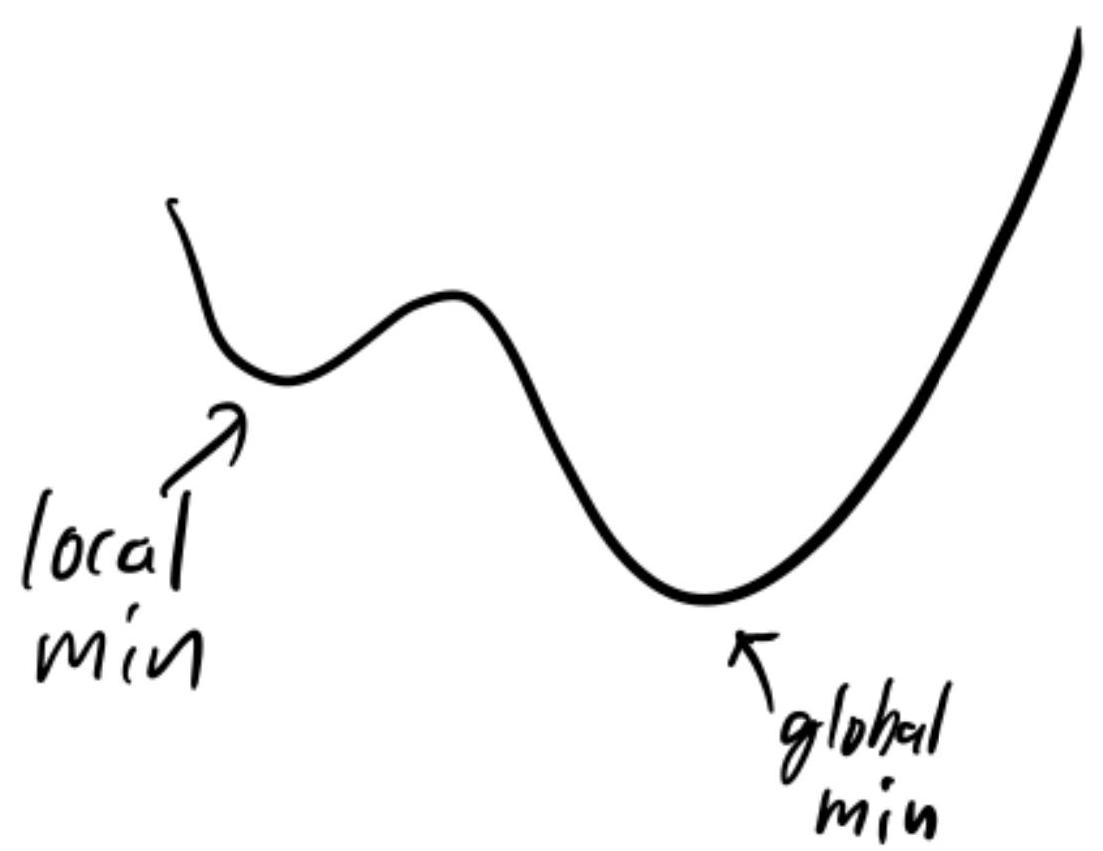
\includegraphics[width=0.5\textwidth]{.././assets/1.1.jpg}
    \end{figure}

    In the worst case, finding the global minimum of an optimization problem is difficult.
    However, in deep learning, optimization problems are often "solved" without any guarantee of global optimality.
\end{definition}
